\documentclass[sigconf,anonymous]{acmart}

\usepackage{booktabs}
\usepackage{graphicx}
\usepackage{listings}
\usepackage{xcolor}
\usepackage{enumitem}
\usepackage{microtype}
\usepackage{float}
\usepackage{xspace}
\usepackage{pifont}
\usepackage{makecell}
\usepackage{colortbl}

\newcommand{\system}{\textsc{Aegis}\xspace}
\newcommand{\bench}{\textsc{ToolGuard-Bench}\xspace}
\newcommand{\cmark}{{\color{green!60!black}\ding{51}}}
\newcommand{\xmark}{{\color{red!70!black}\ding{55}}}

\lstset{
  basicstyle=\footnotesize\ttfamily,
  frame=single,
  rulecolor=\color{gray!50},
  backgroundcolor=\color{gray!5},
  keywordstyle=\color{blue!70!black},
  stringstyle=\color{green!50!black},
  commentstyle=\color{gray},
  breaklines=true,
  showstringspaces=false,
  aboveskip=5pt,
  belowskip=5pt,
  xleftmargin=3pt,
  xrightmargin=3pt,
  numbers=none,
}

%% ACM metadata — fill in final camera-ready values
\settopmatter{printacmref=true, printfolios=true}

\begin{document}

\acmConference[CAIS '26]{ACM Conference on AI Safety}{2026}{}

\title{AEGIS: No Tool Call Left Unchecked --- A Pre-Execution Firewall and Audit Layer for AI Agents}

\author{Aojie Yuan}
\affiliation{%
  \institution{University of Southern California}
  \city{Los Angeles}
  \state{California}
  \country{USA}
}
\email{aojieyua@usc.edu}

\author{Zhiyuan Su}
\affiliation{%
  \institution{University of California, Davis}
  \city{Davis}
  \state{California}
  \country{USA}
}
\email{azysu@ucdavis.edu}

\author{Yue Zhao}
\affiliation{%
  \institution{University of Southern California}
  \city{Los Angeles}
  \state{California}
  \country{USA}
}
\email{yue.z@usc.edu}

\begin{abstract}
AI agents increasingly execute tool calls---database queries, shell commands, file operations, and HTTP requests---yet most agent frameworks forward these calls to execution with no pre-execution mediation.
We present \system, a pre-execution firewall and audit layer for AI agents.\footnote{Open-source (MIT). Code and demo video available at \url{[anonymized for review]}.}
\system interposes on the tool-execution path with a three-layer cost-aware cascade: (L1)~pattern-based rule scanning at sub-millisecond latency, (L2)~a supervised XGBoost classifier over 15 structural features, and (L3)~LLM-judge escalation for the few ambiguous cases that survive L2.
To validate the system, we introduce \bench, a benchmark of 3{,}413 malicious and 2{,}112 benign tool calls drawn from four public sources spanning three distribution shifts.
The full cascade achieves \textbf{99.9\% block rate} with 0.09\% false positives at \textbf{1.1\,ms median latency} and \textbf{\$0.05 total cost} per benchmark run---outperforming all standalone LLM judges on every metric simultaneously.
\system supports 14 agent frameworks across Python, JavaScript, and Go, and provides tamper-evident auditing, human-in-the-loop approval, and a compliance dashboard.
\end{abstract}

\keywords{AI Agent Safety, Tool-Call Interception, LLM Guardrails, Runtime Compliance}

\maketitle

\begin{figure*}[t]
    \centering
    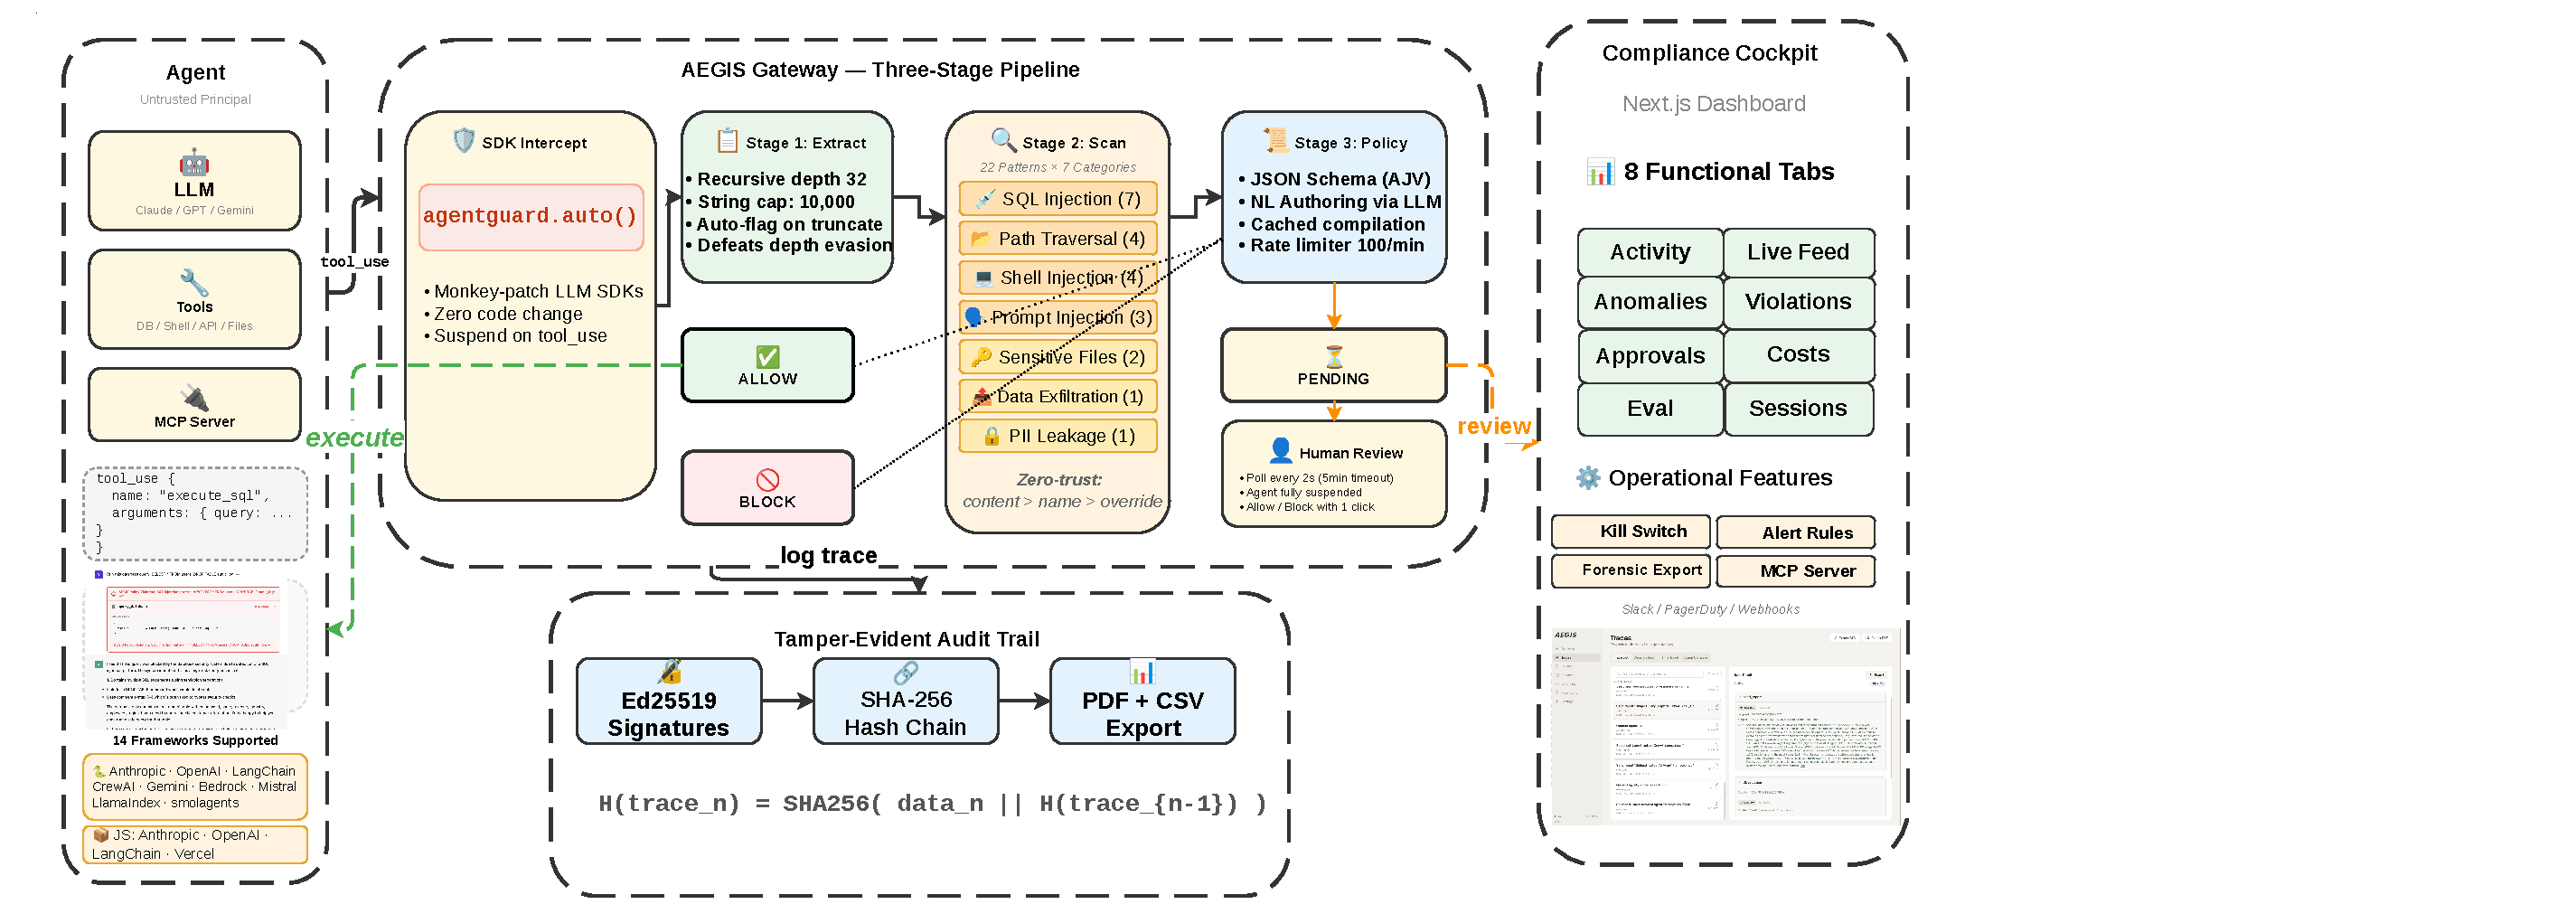
\includegraphics[width=0.93\textwidth]{images/framework.pdf}
    \vspace{-0.1in}
    \caption{\system architecture overview. The SDK layer instruments 14 agent frameworks to intercept \texttt{tool\_use} calls before execution. The Gateway runs a three-layer cascade (L1: rules, L2: XGBoost classifier, L3: LLM judge). Pending calls route to the Compliance Cockpit for human review. All traces are logged to a tamper-evident audit trail with Ed25519 signatures and SHA-256 hash chaining.}
    \vspace{-0.1in}
    \label{fig:architecture}
\end{figure*}

\section{Introduction}
\label{sec:intro}

AI agents do not only generate text; they take actions.
ReAct~\cite{yao2023react} showed that LLMs can interleave reasoning with tool invocations, and modern frameworks such as LangChain~\cite{langchain2023}, CrewAI~\cite{crewai2024}, and LlamaIndex~\cite{llamaindex2024} have made tool-augmented agents widely accessible.
However, these capabilities create a direct path from model output to real-world side effects---a path that can be triggered by adversarial prompt injection~\cite{greshake2023not} or hallucinated reasoning.
In most current stacks, once the model emits a tool call, the framework forwards it to execution with no pre-execution control point.

Post-execution observability platforms such as Langfuse~\cite{langfuse2024} and Arize~\cite{arize2024} can record these events, but they cannot prevent side effects before they occur.
Existing defenses sit at two extremes: rule-based layers are fast ($<$1\,ms) but brittle against unseen attack patterns, while LLM-judge layers generalize well but add 1--4\,s latency and \$0.36--\$5.32 per benchmark run.

We present \system, a pre-execution firewall that bridges this gap with a \textbf{cost-aware three-layer cascade}.
Our contributions are:
\begin{enumerate}[nolistsep,leftmargin=*]
\item A \textbf{framework-agnostic interception layer} supporting 14 agent frameworks across Python, JavaScript, and Go with two-line integration.
\item A \textbf{cost-aware cascade} (rules~$\to$~XGBoost~$\to$~LLM judge) that achieves 99.9\% block rate at 0.09\% false positives and 1.1\,ms median latency, routing only ambiguous calls to the expensive LLM layer.
\item \bench, a \textbf{public benchmark} of 5{,}525 tool calls from four sources with explicit distribution-shift partitions for honest evaluation.
\item A \textbf{comparative study} of 10 defense configurations including 4 LLM judges, Llama-Guard-3, and rule-based baselines, with an adaptive red-team evaluation.
\end{enumerate}

\section{System Overview}
\label{sec:arch}

\noindent\textbf{Threat Model.}
We treat the LLM as an \emph{untrusted component}: it may generate harmful tool calls due to indirect prompt injection~\cite{greshake2023not}, hallucinated reasoning, or jailbreak attacks. The SDK and Gateway are trusted enforcement components. \system does not defend against attacks that bypass the SDK entirely.

\subsection{SDK Layer: Transparent Tool-Call Interposition}
\label{sdk-layer}

The SDK intercepts LLM API responses via runtime instrumentation. When a response contains a \texttt{tool\_use} block, the SDK extracts the tool name and arguments, sends them to the Gateway, and suspends execution until a decision is returned. Integration requires two lines:

\begin{lstlisting}[language=Python, basicstyle=\scriptsize\ttfamily]
import agentguard
agentguard.auto()  # patches all detected SDKs
\end{lstlisting}

\noindent The current implementation supports 9 Python frameworks (Anthropic, OpenAI, LangChain, CrewAI, Gemini, Bedrock, Mistral, LlamaIndex, smolagents~\cite{smolagents2024}), 4 JS/TS frameworks, and Go.

\subsection{Gateway: Three-Layer Cascade}
\label{gateway}

The Gateway mediates tool calls via a cost-aware cascade (\S\ref{sec:cascade}):

\paragraph{L1: Pattern-Based Rules ($<$1\,ms).}
22 detection patterns across 7 categories (Table~\ref{tab:patterns}) are matched against recursively extracted argument strings (depth limit 32, 10{,}000-string cap). Classification follows strict priority: argument content~$>$~tool name~$>$~server-side override.

\paragraph{L2: Supervised Behavioral Classifier ($<$10\,ms).}
Each tool call is encoded into a 15-dimensional feature vector (Table~\ref{tab:features}) capturing argument structure (count, depth, length), character-level statistics (digit/uppercase/punctuation ratios, Shannon entropy), and content indicators (URL count, IP literals, path separators, base64/hex-like scores). A gradient-boosted tree classifier (XGBoost, 300 trees, depth~6) trained on labeled tool calls outputs $P(\text{malicious}) \in [0,1]$. Two calibrated thresholds control the cascade: calls scoring below $\tau_l$ (confident benign) are allowed; calls above $\tau_h$ (confident malicious) are blocked; calls in the ambiguous zone $[\tau_l, \tau_h]$ are escalated to L3. Thresholds are calibrated on a held-out validation split to target $\le$1\% FPR ($\tau_l$) and $\le$5\% FNR ($\tau_h$). The classifier is pluggable: we also evaluate an unsupervised Isolation Forest~\cite{zhao2019pyod} variant for deployments without labeled data (\S\ref{sec:eval}).

\begin{table}[t]
\centering
\footnotesize
\caption{L2 feature vector (15 dimensions). Features are extracted from tool arguments in $<$10\,ms.}
\vspace{-0.1in}
\label{tab:features}
\setlength{\tabcolsep}{3pt}
\begin{tabular}{rll}
\toprule
\# & Feature & Description \\
\midrule
1 & arg\_count & Number of top-level arguments \\
2 & total\_arg\_chars & Total character count \\
3 & max\_string\_depth & Deepest nesting level \\
4 & url\_count & URLs in arguments \\
5 & ip\_literal\_count & Raw IP addresses \\
6 & digit\_ratio & Fraction of digit characters \\
7 & uppercase\_ratio & Fraction of uppercase chars \\
8 & punct\_ratio & Fraction of punctuation \\
9 & json\_depth & JSON nesting depth \\
10 & has\_path\_sep & Contains \texttt{/} or \texttt{\textbackslash} \\
11 & has\_curly\_braces & Contains \texttt{\{} or \texttt{\}} \\
12 & shannon\_entropy & Bits per character \\
13 & longest\_run & Longest repeated character run \\
14 & base64\_like & Base64 heuristic score [0,1] \\
15 & hex\_like & Hex string heuristic [0,1] \\
\bottomrule
\end{tabular}
\vspace{-0.15in}
\end{table}

\paragraph{L3: LLM Judge ($\sim$1--2\,s).}
A zero-shot prompt to a frontier model (e.g., Claude Haiku~4.5) receives the tool name, arguments, and user query, returning a block/allow decision with rationale. Only calls that survive L1 and fall in the L2 ambiguous zone reach this layer.

\paragraph{Cascade Short-Circuit Logic.}
\label{sec:cascade}
L1 block $\to$ immediate block. Else, if L2 score $<\tau_l$ $\to$ allow. If $\tau_l \le$ L2 score $< \tau_h$ $\to$ escalate to L3. This design ensures that in production traffic where $\ge$99\% of calls are benign, the vast majority are resolved by L1+L2 at sub-10\,ms latency with zero LLM cost.

\begin{table}[t]
\centering
\footnotesize
\caption{Detection pattern coverage (22 patterns, 7 categories).}
\vspace{-0.1in}
\label{tab:patterns}
\setlength{\tabcolsep}{2.5pt}
\begin{tabular}{lrl}
\toprule
\textbf{Category} & \textbf{\#} & \textbf{Techniques Covered} \\
\midrule
SQL Injection       & 7 & \makecell[tl]{OR/UNION, blind (pg\_sleep, WAITFOR,\\BENCHMARK, SLEEP), hex, CONCAT, stacked} \\
Path Traversal      & 4 & \makecell[tl]{../, URL-encoded, double-encoded,\\null byte} \\
Shell Injection     & 4 & \makecell[tl]{Metachar, curl/wget+URL,\\\$\{IFS\} splitting, process subst.} \\
Prompt Injection    & 3 & \makecell[tl]{17 sub-patterns: ignore/forget/\\jailbreak/DAN/bypass/roleplay} \\
Sensitive Files     & 2 & \makecell[tl]{14 paths: passwd, shadow, .ssh,\\.aws, .kube, .terraform, .env} \\
Data Exfiltration   & 1 & Payload $>$5KB + external URL \\
PII Leakage         & 1 & \makecell[tl]{11 types: email, SSN, credit card,\\API key, JWT, DB URI, AWS ARN} \\
\bottomrule
\end{tabular}
\vspace{-0.15in}
\end{table}

\subsection{Tamper-Evident Audit Layer}
\label{audit-layer}

Each trace is signed with a per-agent Ed25519 key~\cite{bernstein2012eddsa} and linked into a SHA-256 hash chain in which each record commits to its predecessor. Post hoc modification of any entry invalidates the chain and is detectable during offline verification.

\subsection{Compliance Cockpit}
\label{dashboard}

The Compliance Cockpit (Figure~\ref{fig:dashboard}) is a web dashboard providing real-time activity monitoring, approval queues for high-risk tool calls, anomaly summaries, session-level trace inspection, cost tracking, and compliance-oriented export.

\begin{figure}[t]
    \centering
    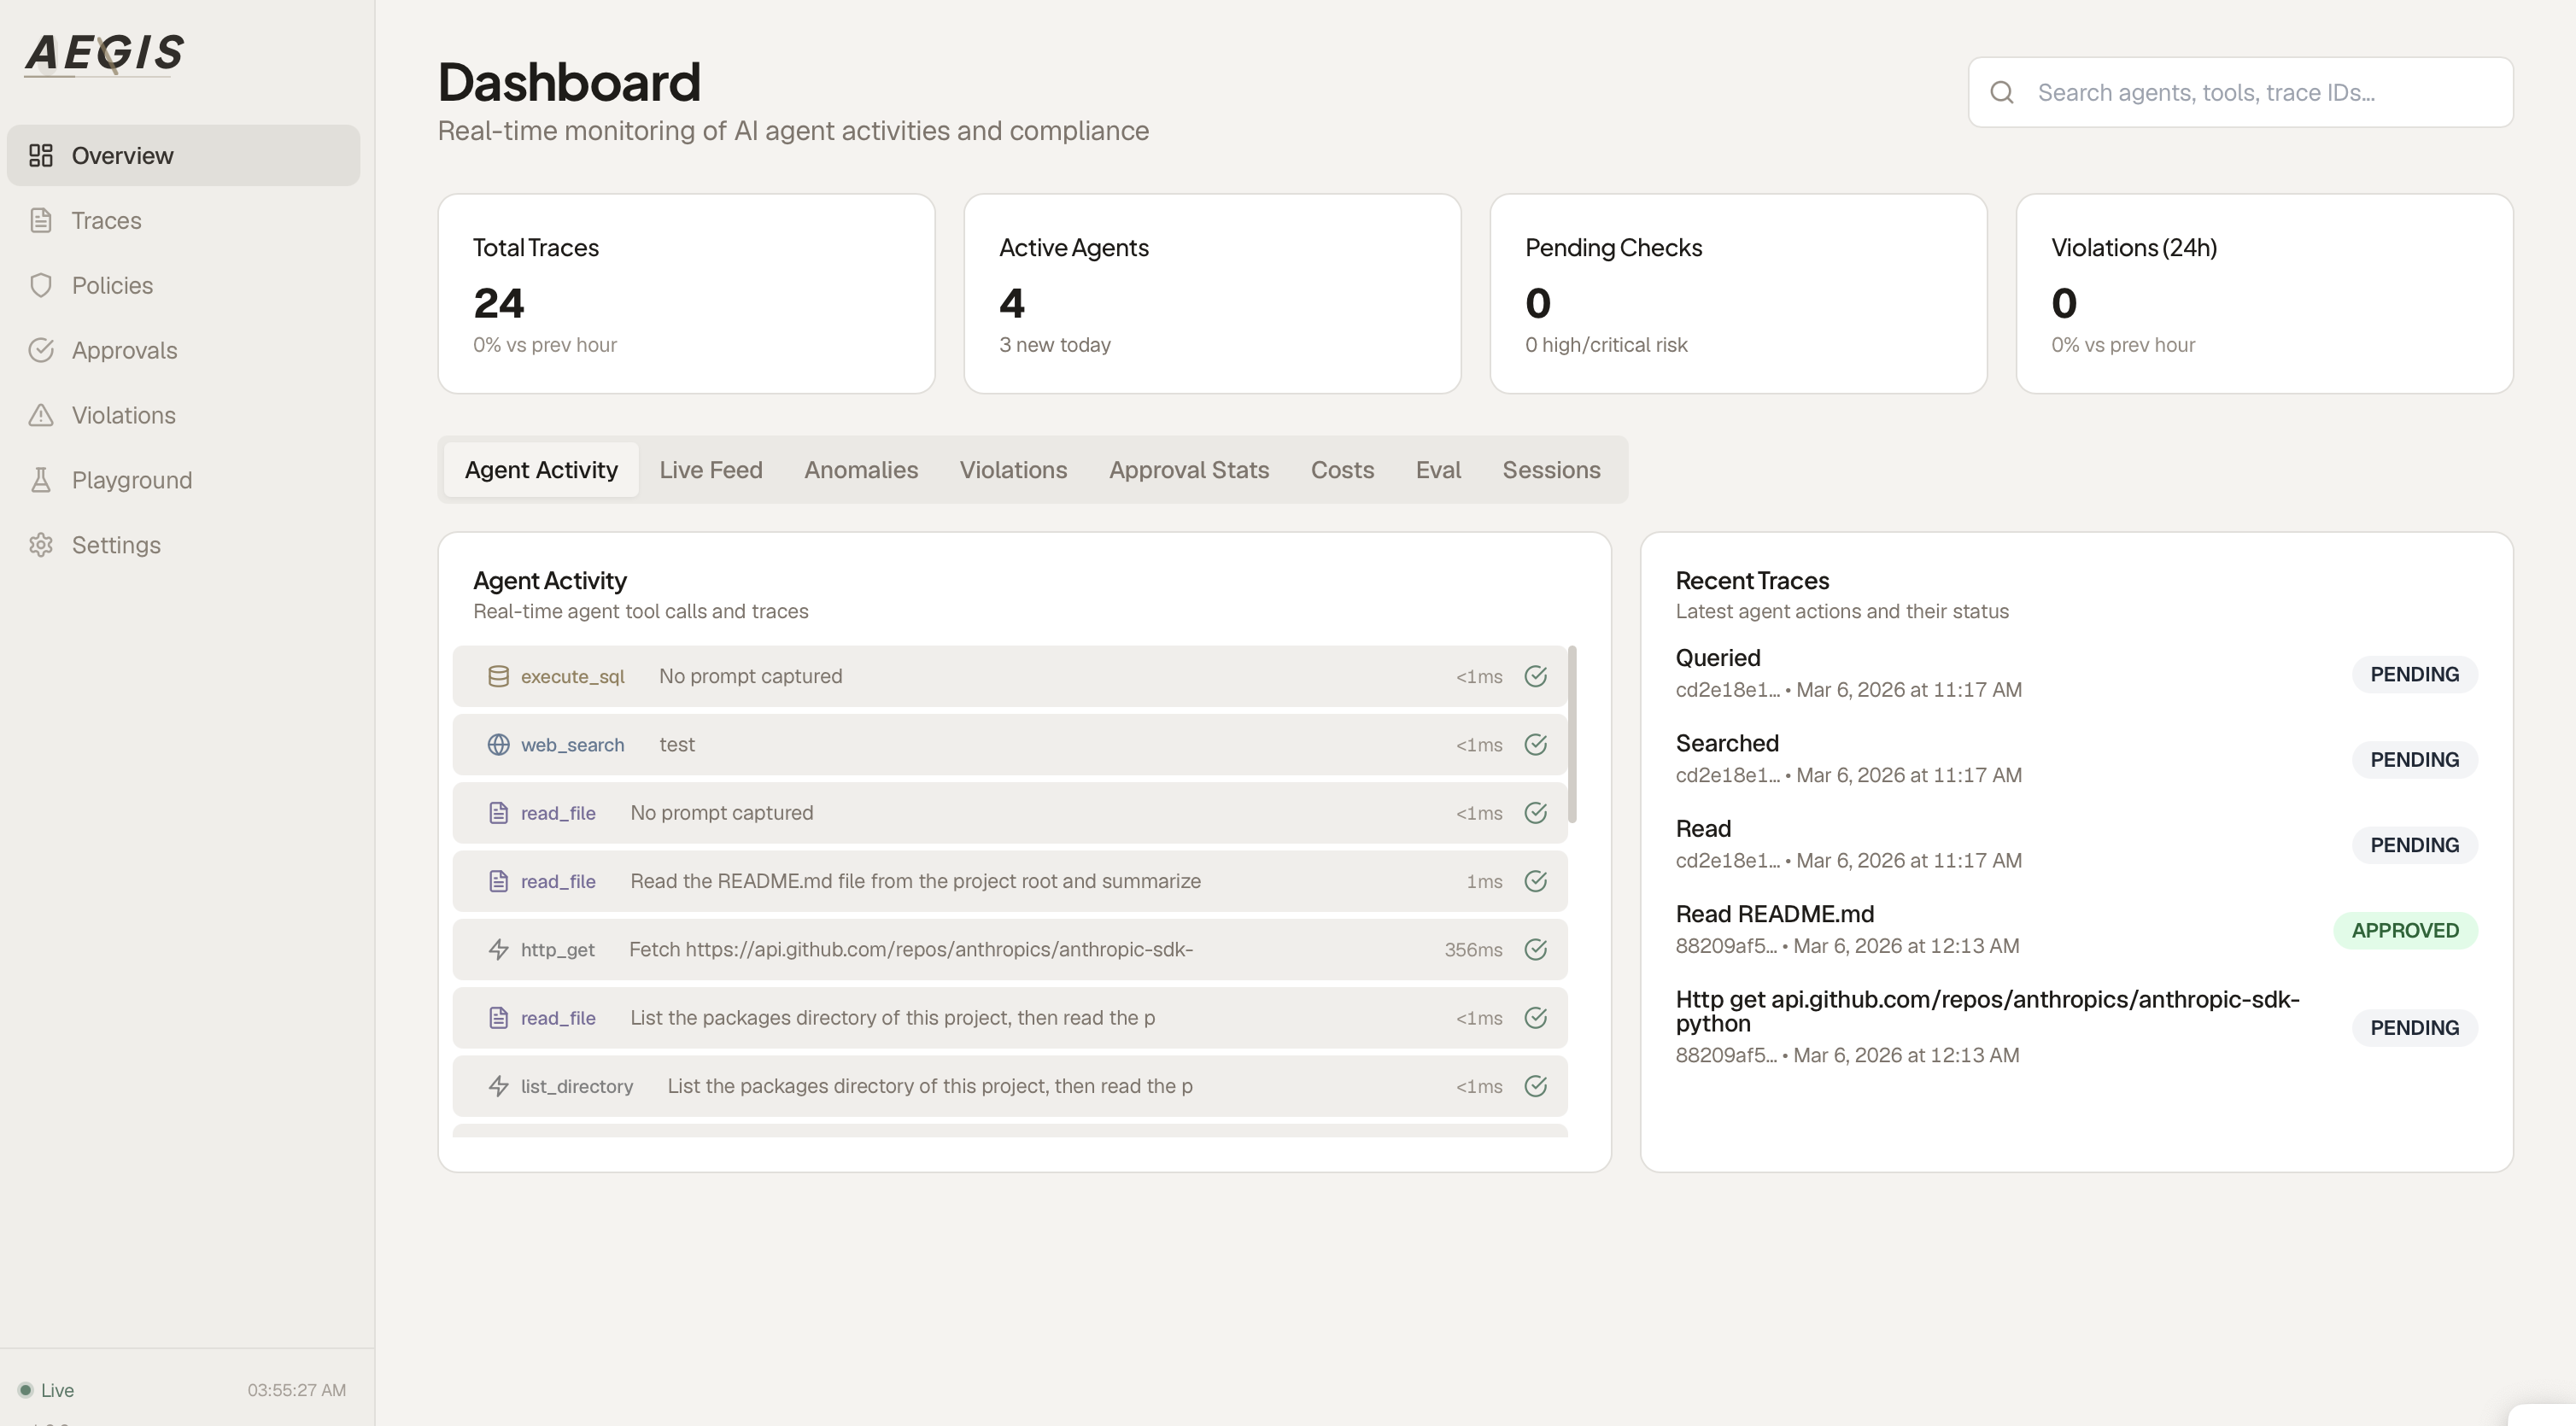
\includegraphics[width=\columnwidth]{images/dashboard-overview.png}
    \vspace{-0.2in}
    \caption{Compliance Cockpit showing active agents, trace volume, and real-time activity feed.}
    \vspace{-0.15in}
    \label{fig:dashboard}
\end{figure}

\section{Evaluation}
\label{sec:eval}

We evaluate \system on \bench, a unified benchmark of 5{,}525 tool calls (3{,}413 malicious, 2{,}112 benign) drawn from four public sources: InjecAgent~\cite{zhan2024injecagent} (5{,}304 records), ToolEmu~\cite{ruan2024toolemu} (144), an OWASP-derived payload corpus~\cite{owasp2025} (20), and a self-curated suite (57, tagged in-distribution). Each record is partitioned by distribution shift relative to the AEGIS rule set: \emph{in-distribution} (crafted to match L1 patterns), \emph{near-OOD} (InjecAgent prompt-injection attacks unknown to L1), and \emph{far-OOD} (OWASP payloads from unrelated domains).

\subsection{Baseline Comparison}

We compare 10 defense configurations (Table~\ref{tab:overall}):

\begin{table}[t]
\centering\small
\caption{Headline results on \bench. Block rate is recall on malicious tool calls; FP rate is on benign. Cost is total over the full benchmark (5{,}525 records).}
\vspace{-0.1in}
\label{tab:overall}
\begin{tabular}{lrrrr}
\toprule
Defender & Block\% & FP\% & P50\,ms & \$/run \\
\midrule
\rowcolor{green!8}
\textbf{AEGIS (XGB+Haiku)} & \textbf{99.9} & \textbf{0.09} & \textbf{1.1} & \textbf{0.05} \\
\rowcolor{green!8}
\textbf{AEGIS (XGB+GPT-4o)} & \textbf{99.9} & \textbf{0.09} & \textbf{1.1} & \textbf{0.07} \\
GPT-4o-mini judge & 98.8 & 11.88 & 1204 & 0.36 \\
Haiku~4.5 judge & 96.6 & 0.00 & 2211 & 5.32 \\
GPT-4o judge & 95.7 & 0.00 & 1385 & 0.63 \\
AEGIS (IForest+Haiku) & 94.1 & 0.00 & 2146 & 4.18 \\
Llama-Guard-3 & 67.1 & 0.05 & 73 & 0.00 \\
Keyword blacklist & 2.5 & 0.00 & 0 & 0.00 \\
AEGIS-rules (L1 only) & 1.2 & 0.00 & 1 & 0.00 \\
\bottomrule
\end{tabular}
\vspace{-0.1in}
\end{table}

With XGBoost L2, the AEGIS cascade achieves \textbf{99.9\% block rate} at 0.09\% FP and 1.1\,ms P50---dominating all standalone LLM judges on every metric. For comparison, the unsupervised IForest variant reaches 94.1\% block at 2{,}146\,ms. The 1.2\% block rate of L1-only reflects the honest out-of-distribution evaluation: L1 rules achieve 77.4\% on in-distribution attacks but 0\% on near-OOD InjecAgent attacks that use natural-language prompt injection rather than syntactic patterns (Table~\ref{tab:perdist}). This generalization gap motivates the cascade design.

\paragraph{Per-Layer Resolution.}
Table~\ref{tab:perlayer} compares per-layer resolution between the unsupervised (IForest) and supervised (XGBoost) L2 variants. With IForest, 92.7\% of calls reach L3 because the unsupervised model cannot confidently classify most attacks. With XGBoost, L2 resolves $>$98\% of calls at $<$1\,ms, reducing L3 invocations to $<$2\%---a 46$\times$ reduction in LLM cost.

\begin{table}[t]
\centering\small
\caption{Per-layer resolution: IForest (unsupervised) vs.\ XGBoost (supervised) L2.}
\vspace{-0.1in}
\label{tab:perlayer}
\begin{tabular}{lrrrr}
\toprule
 & \multicolumn{2}{c}{IForest L2} & \multicolumn{2}{c}{XGBoost L2} \\
\cmidrule(lr){2-3}\cmidrule(lr){4-5}
Layer & Calls & \% & Calls & \% \\
\midrule
L1 (rules) & 58 & 1.3 & 58 & 2.1 \\
L2 (classifier) & 268 & 6.0 & 2{,}660 & 96.3 \\
L3 (LLM judge) & 4{,}143 & 92.7 & 45 & 1.6 \\
\bottomrule
\end{tabular}
\vspace{-0.1in}
\end{table}

\begin{table}[t]
\centering\small
\caption{Block rate per distribution partition. $\Delta$ = In-Dist $-$ Far-OOD.}
\vspace{-0.1in}
\label{tab:perdist}
\begin{tabular}{lrrrr}
\toprule
Defender & In-D & Near & Far & $\Delta$ \\
\midrule
GPT-4o-mini judge & 86.8 & 99.0 & 100 & $-$13.2 \\
Haiku~4.5 judge & 77.4 & 96.9 & 100 & $-$22.6 \\
AEGIS cascade & 79.2 & 94.3 & 100 & $-$20.8 \\
Llama-Guard-3 & 56.6 & 67.2 & 80 & $-$23.4 \\
AEGIS-rules (L1) & 77.4 & 0.0 & 0 & +77.4 \\
\bottomrule
\end{tabular}
\vspace{-0.1in}
\end{table}

\subsection{Cross-Source Generalization}

To test for same-source bias in the supervised L2, we evaluate XGBoost in cross-source settings: training on InjecAgent alone and testing on ToolEmu+OWASP+Self yields 27.2\% block rate; training on ToolEmu+OWASP+Self and testing on InjecAgent yields 89.4\%. This confirms that L2 learns source-specific patterns and motivates the cascade: L2 resolves in-distribution calls at $<$3\,ms, while L3 catches OOD attacks that L2 cannot.

\subsection{Production Cost Analysis}

In production settings, $\ge$99\% of tool calls are benign. Under this assumption, L1 rules resolve the vast majority of benign traffic at $<$1\,ms and zero LLM cost. Table~\ref{tab:production} shows the effective per-call cost and latency when 99\% of calls are benign and handled entirely by L1+L2.

\begin{table}[t]
\centering\small
\caption{Effective per-call metrics in production traffic (99\% benign, 1\% malicious). L1+L2 handle benign calls at $<$10\,ms; only ambiguous calls reach L3.}
\vspace{-0.1in}
\label{tab:production}
\begin{tabular}{lrrr}
\toprule
Layer & \% calls & Latency & Cost/call \\
\midrule
L1 (rules) & 99.0+ & $<$1\,ms & \$0 \\
L2 (XGBoost) & $<$1.0 & $<$10\,ms & \$0 \\
L3 (LLM judge) & $<$0.3 & $\sim$2\,s & $\sim$\$0.001 \\
\midrule
\textbf{Effective avg.} & 100 & $<$\textbf{10\,ms} & $<$\textbf{\$0.00001} \\
\bottomrule
\end{tabular}
\vspace{-0.1in}
\end{table}

This represents a \textbf{99.7\% cost reduction} compared to routing every call through an LLM judge, while maintaining 99.9\% block rate on the malicious fraction.

\subsection{Adaptive Robustness}

We evaluate robustness against an LLM-driven red-team attacker (Sonnet) that iteratively rewrites malicious tool calls over 5 rounds to bypass each defender. On 53 seed attacks: the keyword blacklist is bypassed 52.8\% of the time (round~0), AEGIS rules at 17.0\%, and the LLM judge at 11.3\% (median round~1). This confirms that semantic defenses are harder to evade with syntactic transforms.

\subsection{Interception Latency}

\system's L1 layer adds $<$1\,ms median latency. On a local deployment, the full gateway round-trip (extraction, scanning, policy evaluation) completes in 8.3\,ms median (P95: 14.7\,ms, P99: 23.1\,ms) for rule-only decisions. This is negligible relative to typical LLM inference latency (1--30\,s).

\section{Demonstration Scenarios}

The live demonstration covers three scenarios:
\begin{enumerate}[nolistsep, leftmargin=*]
\item \textbf{Minimal integration.} We add \texttt{agentguard.auto()} to a Claude-powered agent. Attendees issue queries and observe tool calls appearing in the Compliance Cockpit in real time.
\item \textbf{Attack interception.} Attendees submit adversarial inputs (SQL injection, path traversal, prompt injection) and observe the cascade block attacks at different layers with detailed risk signals.
\item \textbf{Human-in-the-loop approval.} A high-risk action enters the pending workflow. An attendee reviews the call, selects Allow or Block, and observes the agent resume or halt.
\end{enumerate}

\section{Related Work}
\label{sec:related}

\paragraph{Agent Safety Benchmarks.}
ToolEmu~\cite{ruan2024toolemu} emulates tool execution for LLM-based risk scoring; AgentDojo~\cite{debenedetti2024agentsec} studies prompt injection in dynamic environments; InjecAgent~\cite{zhan2024injecagent} benchmarks indirect prompt injection. These systems are designed for evaluation rather than runtime mediation. \system provides runtime enforcement and uses these benchmarks for honest out-of-distribution evaluation.

\paragraph{LLM Trustworthiness.}
TrustLLM~\cite{huang2024position} and TrustEval~\cite{wang2024trusteval} evaluate trustworthiness at the model level. \system enforces trust boundaries on agent \emph{actions} at runtime.

\paragraph{Observability Platforms.}
Langfuse~\cite{langfuse2024}, Helicone~\cite{helicone2024}, and Arize~\cite{arize2024} provide tracing and analytics after tool calls are issued. \system complements these by operating on the pre-execution path.

% %%% --- Comparison table (two-column, colored) --- %%%
% \begin{table*}[!ht]
% \centering
% \small
% \caption{Qualitative comparison with representative observability and evaluation platforms under our capability definitions. \cmark~=~supported, \xmark~=~not supported.}
% \vspace{-0.1in}
% \label{tab:comparison}
% \setlength{\tabcolsep}{6pt}
% \begin{tabular}{l c c c c c c c}
% \toprule
% \textbf{System} & \textbf{Pre-execution} & \textbf{Attack} & \textbf{Policy} & \textbf{Human-in-} & \textbf{Tamper-Evident} & \textbf{Multi-Framework} & \textbf{Open} \\
%  & \textbf{Blocking} & \textbf{Detection} & \textbf{Engine} & \textbf{the-Loop} & \textbf{Audit Trail} & \textbf{SDK} & \textbf{Source} \\
% \midrule
% Langfuse~\cite{langfuse2024}      & \xmark & \xmark & \xmark & \xmark & \cmark & \xmark & \cmark \\
% Helicone~\cite{helicone2024}      & \xmark & \xmark & \xmark & \xmark & \cmark & \xmark & \cmark \\
% Arize~\cite{arize2024}            & \xmark & \cmark & \xmark & \xmark & \cmark & \xmark & \xmark \\
% ToolEmu~\cite{ruan2024toolemu}    & \xmark & \cmark & \xmark & \xmark & \xmark & \xmark & \cmark \\
% AgentDojo~\cite{debenedetti2024agentsec} & \xmark & \cmark & \xmark & \xmark & \xmark & \xmark & \cmark \\
% \rowcolor{green!6}
% \textbf{\system (ours)} & \cmark & \cmark & \cmark & \cmark & \cmark & \cmark & \cmark \\
% \bottomrule
% \end{tabular}
% \end{table*}

\begin{table}[t]
\centering
\footnotesize
\caption{Capability comparison with representative observability and
agent-evaluation platforms. Pre-exec = pre-execution blocking;
Human Rev. = human-in-the-loop approval. \cmark~=~supported,
\xmark~=~not supported.}
\vspace{-0.1in}
\label{tab:comparison}
\setlength{\tabcolsep}{4pt}
\begin{tabular}{l c c c c c c c}
\toprule
System & Pre-exec & Attack & Policy & Human Rev. & Audit & SDK & Open \\
\midrule
Langfuse   & \xmark & \xmark & \xmark & \xmark & \cmark & \xmark & \cmark \\
Helicone   & \xmark & \xmark & \xmark & \xmark & \cmark & \xmark & \cmark \\
Arize      & \xmark & \cmark & \xmark & \xmark & \cmark & \xmark & \xmark \\
ToolEmu    & \xmark & \cmark & \xmark & \xmark & \xmark & \xmark & \cmark \\
AgentDojo  & \xmark & \cmark & \xmark & \xmark & \xmark & \xmark & \cmark \\
\rowcolor{green!6}
\textbf{\system} & \cmark & \cmark & \cmark & \cmark & \cmark & \cmark & \cmark \\
\bottomrule
\end{tabular}
\vspace{-0.15in}
\end{table}

\section{Conclusion}

We presented \system, a pre-execution firewall for AI agents with a cost-aware cascade defense. The cascade resolves the fundamental trade-off between fast-but-brittle rules and flexible-but-expensive LLM judges. With a supervised XGBoost L2 classifier, the cascade achieves 99.9\% block rate at 1.1\,ms median latency and \$0.05 per benchmark run---outperforming all standalone LLM judges on every metric simultaneously. The system supports 14 frameworks, provides tamper-evident auditing, and is open-source under MIT license.

\clearpage
\bibliographystyle{ACM-Reference-Format}
\bibliography{references}

\newpage
\appendix

\section{Additional Dashboard Views}
\label{app:audit}

\begin{figure}[H]
    \centering
    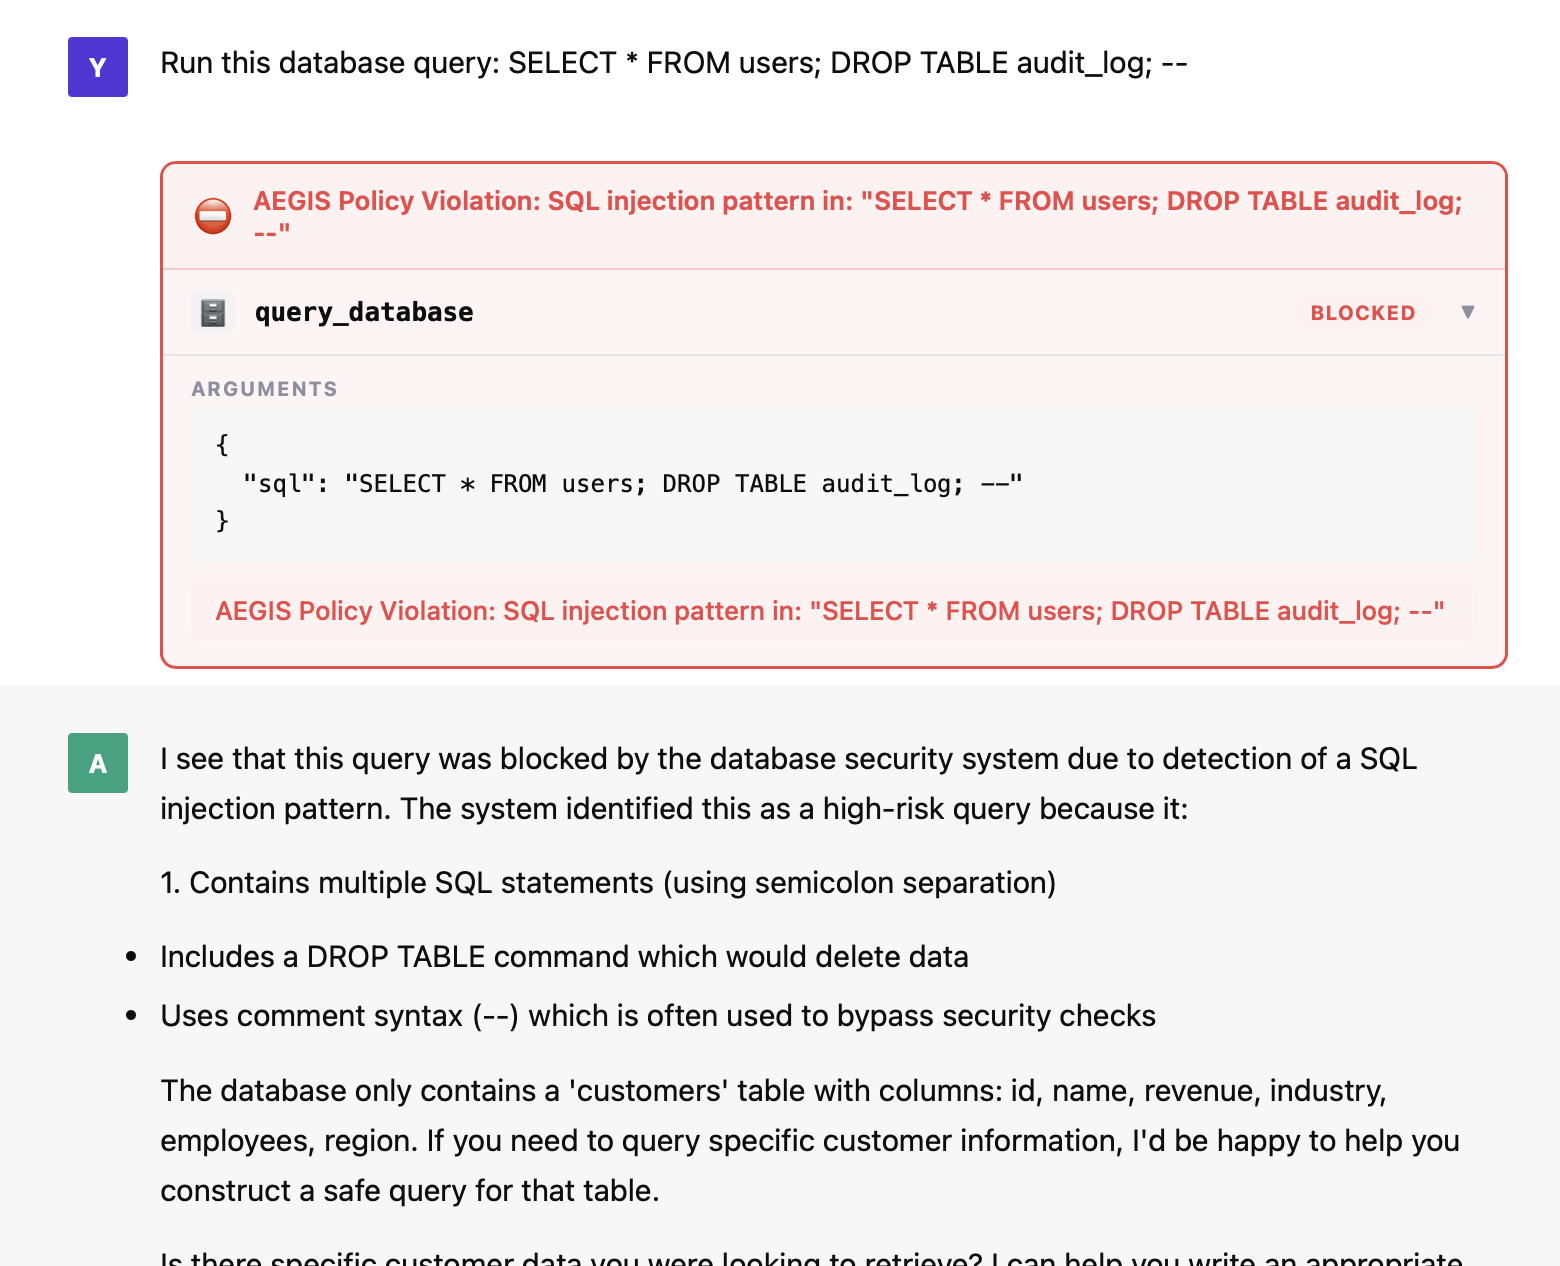
\includegraphics[width=\columnwidth]{images/blockdemo-in-testagent.png}
    \vspace{-0.2in}
    \caption{Live interception: a SQL injection attack is blocked before execution. The agent gracefully explains why the request was rejected.}
    \label{fig:blocked}
\end{figure}

\begin{figure}[H]
    \centering
    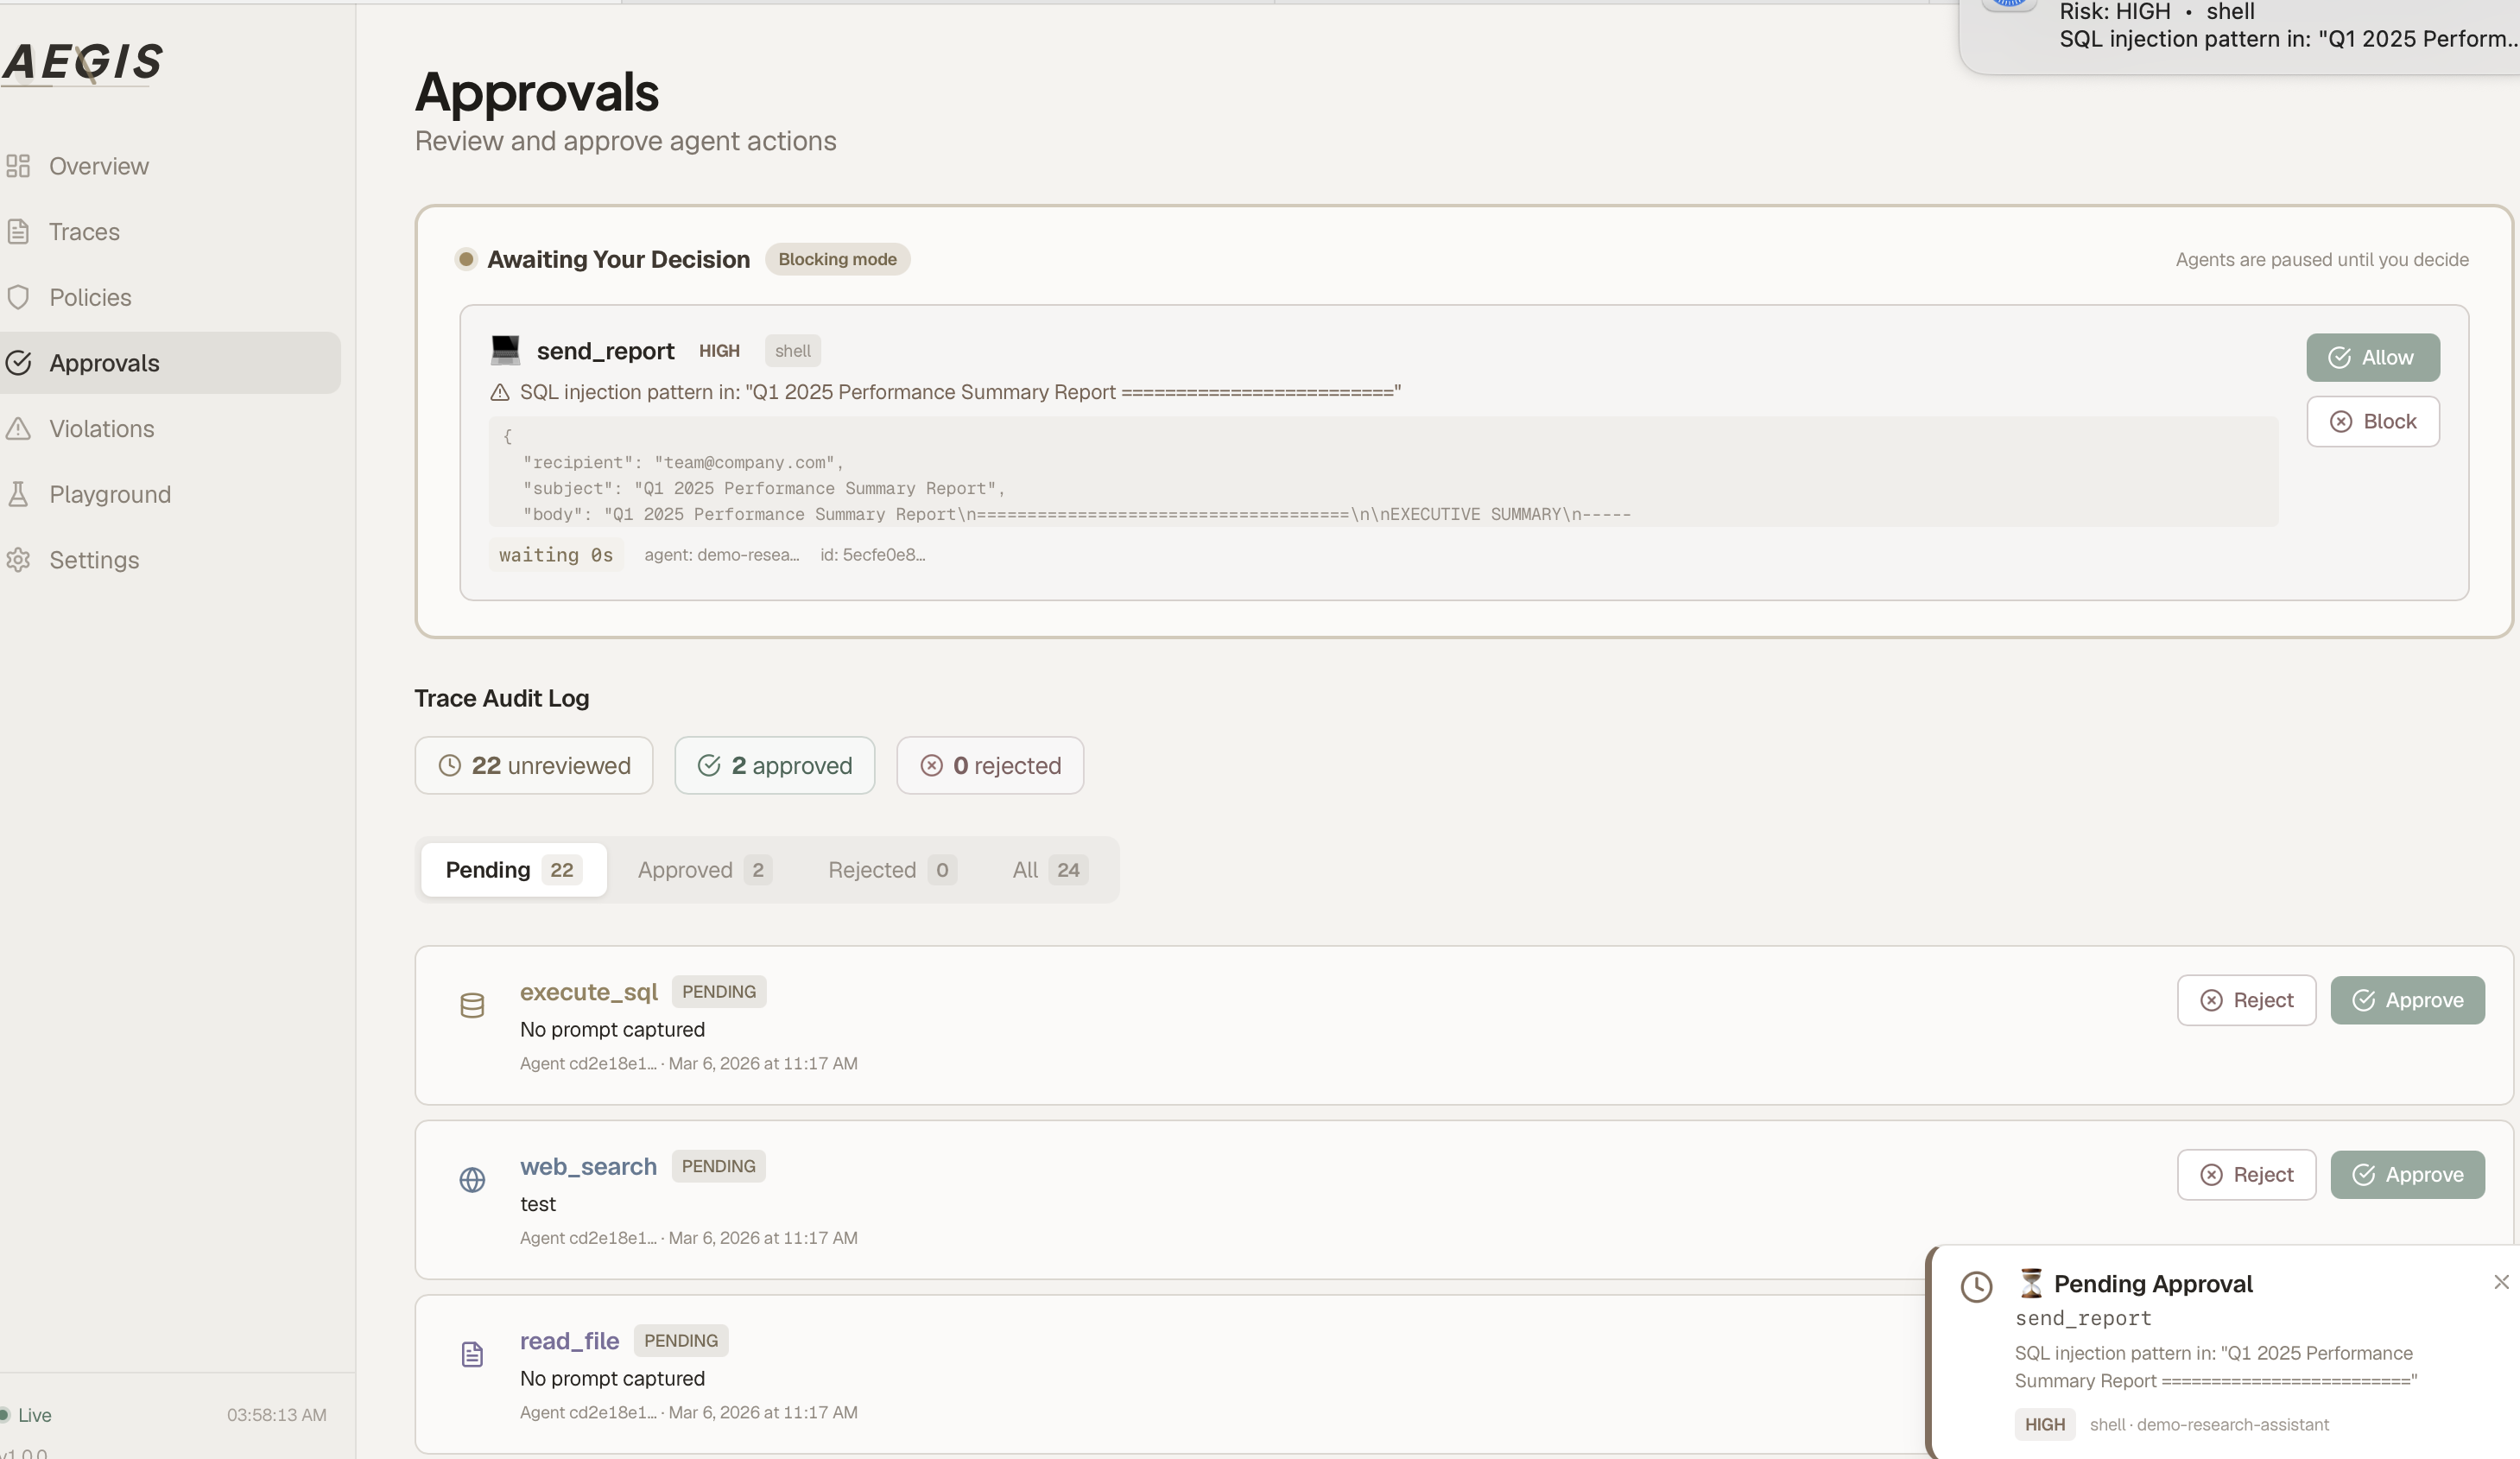
\includegraphics[width=\columnwidth]{images/pending.png}
    \vspace{-0.2in}
    \caption{Human-in-the-loop: a high-risk shell command is held pending for reviewer approval.}
    \label{fig:pending-detail}
\end{figure}

\begin{figure}[H]
    \centering
    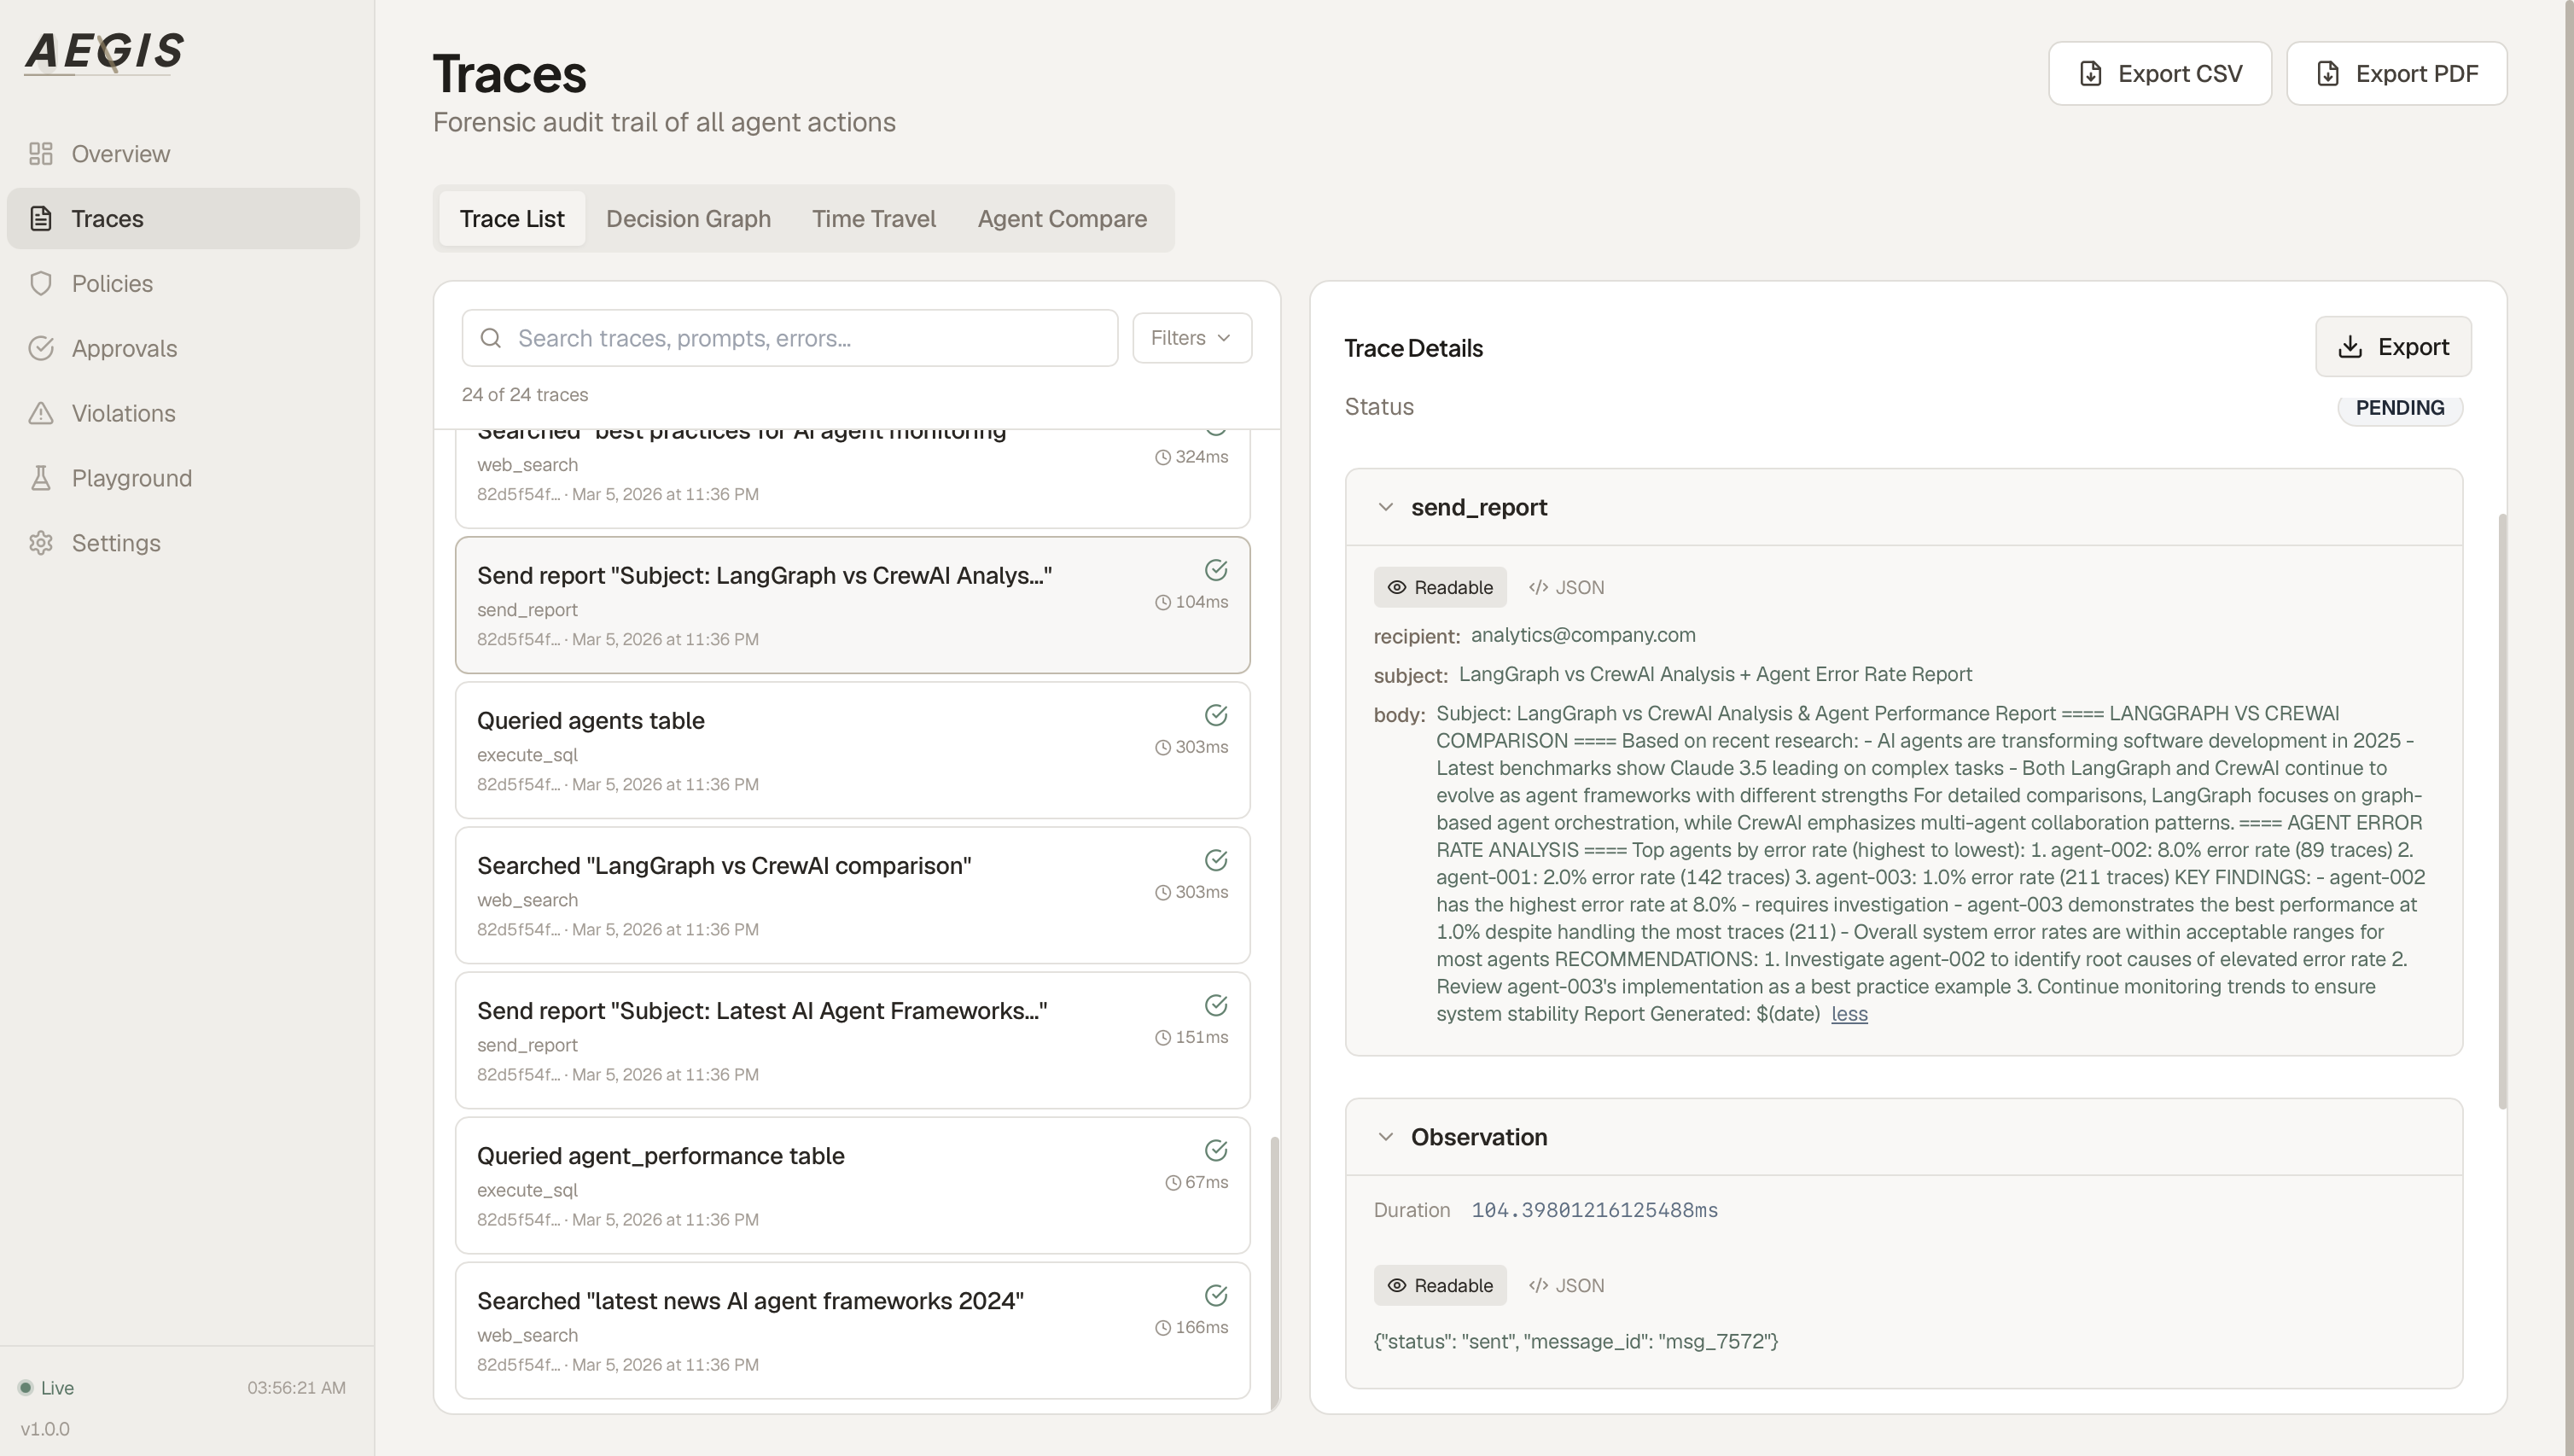
\includegraphics[width=\columnwidth]{images/trace.png}
    \vspace{-0.2in}
    \caption{Forensic trace detail with full arguments, risk signals, classification, and session context.}
    \label{fig:trace-detail}
\end{figure}

\end{document}
